\graphicspath{{Images/intro/}}
\chapter{introduction}
\label{chap:intro}
Traditionally, robots are made of rigid materials such as steel. Rigidity enables such robots to perform repeated tasks with high speed and precision. Rigid robots such as the ones used in car manufacturing assembly lines, are usually designed for specific tasks and they are therefore, less applicable in the presence of changes in the working conditions. Biological organisms on the other hand, can perform a wide range of tasks, although with lower precision and speed. Scientists have thus been investigating using soft materials in robots mimic soft living organisms in terms of their adaptability.~\subfigref{fig:venn}{a} shows an example of a soft robot that can perform grasping of delicate objects without damaging them, regardless of their shape or surface roughness~\cite{Li2019}.

Untethered robots are a class of robots that can function independently without any connection to external power supplies or other equipment. Therefore, untethered robots can be used as autonomous mobile robots in remote locations or in situation where the robot needs to move around and perform tasks such as in factory floors or in warehouses. Boston Dynamics' Atlas\footnote{https://www.bostondynamics.com/atlas\label{fn:boston}} can be considered as an example of untethered robots as can be seen in~\subfigref{fig:venn}{b}. 

Miniature robot applications include exploring tight spaces like the human body. Since miniature robots use less material, and the fabrication processes for making miniature robots often utilize precision tooling, automation, or processes that are easily parallelized,and their fabrication methods are less costly, they can be manufactured in large scale and be used in swarm robotics. The mentioned three categories of robots can be combined to make robots that have the advantages of each.~\subfigref{fig:venn}{c,d,e} highlight examples of such robots.One example shown in~\subfigref{fig:venn}{c} shows a low cost miniature insect-inspired robot that can be used in large numbers to pollinate plants~\cite{Jafferis2019}. 

Miniature, untethered soft robots take advantage of all categories and are the focus of this dissertation as shown in~\subfigref{fig:venn}{f}~\cite{Khodambashi2021untethered}. In this chapter, a brief survey of soft robot technologies is presented. Then, the state of the art in miniature robots is discussed and the limitations of current miniature soft robots is presented. Finally, the contributions of this dissertation which aims at solving some of the challenges are summarized.
 
%In this chapter, the reasons that justify the use of soft robots are discussed. Then the limitations of current soft robot technologies are presented, followed by an overview of the problems that are addressed by this thesis. 
\begin{figure*}[!ht]
      \centering
      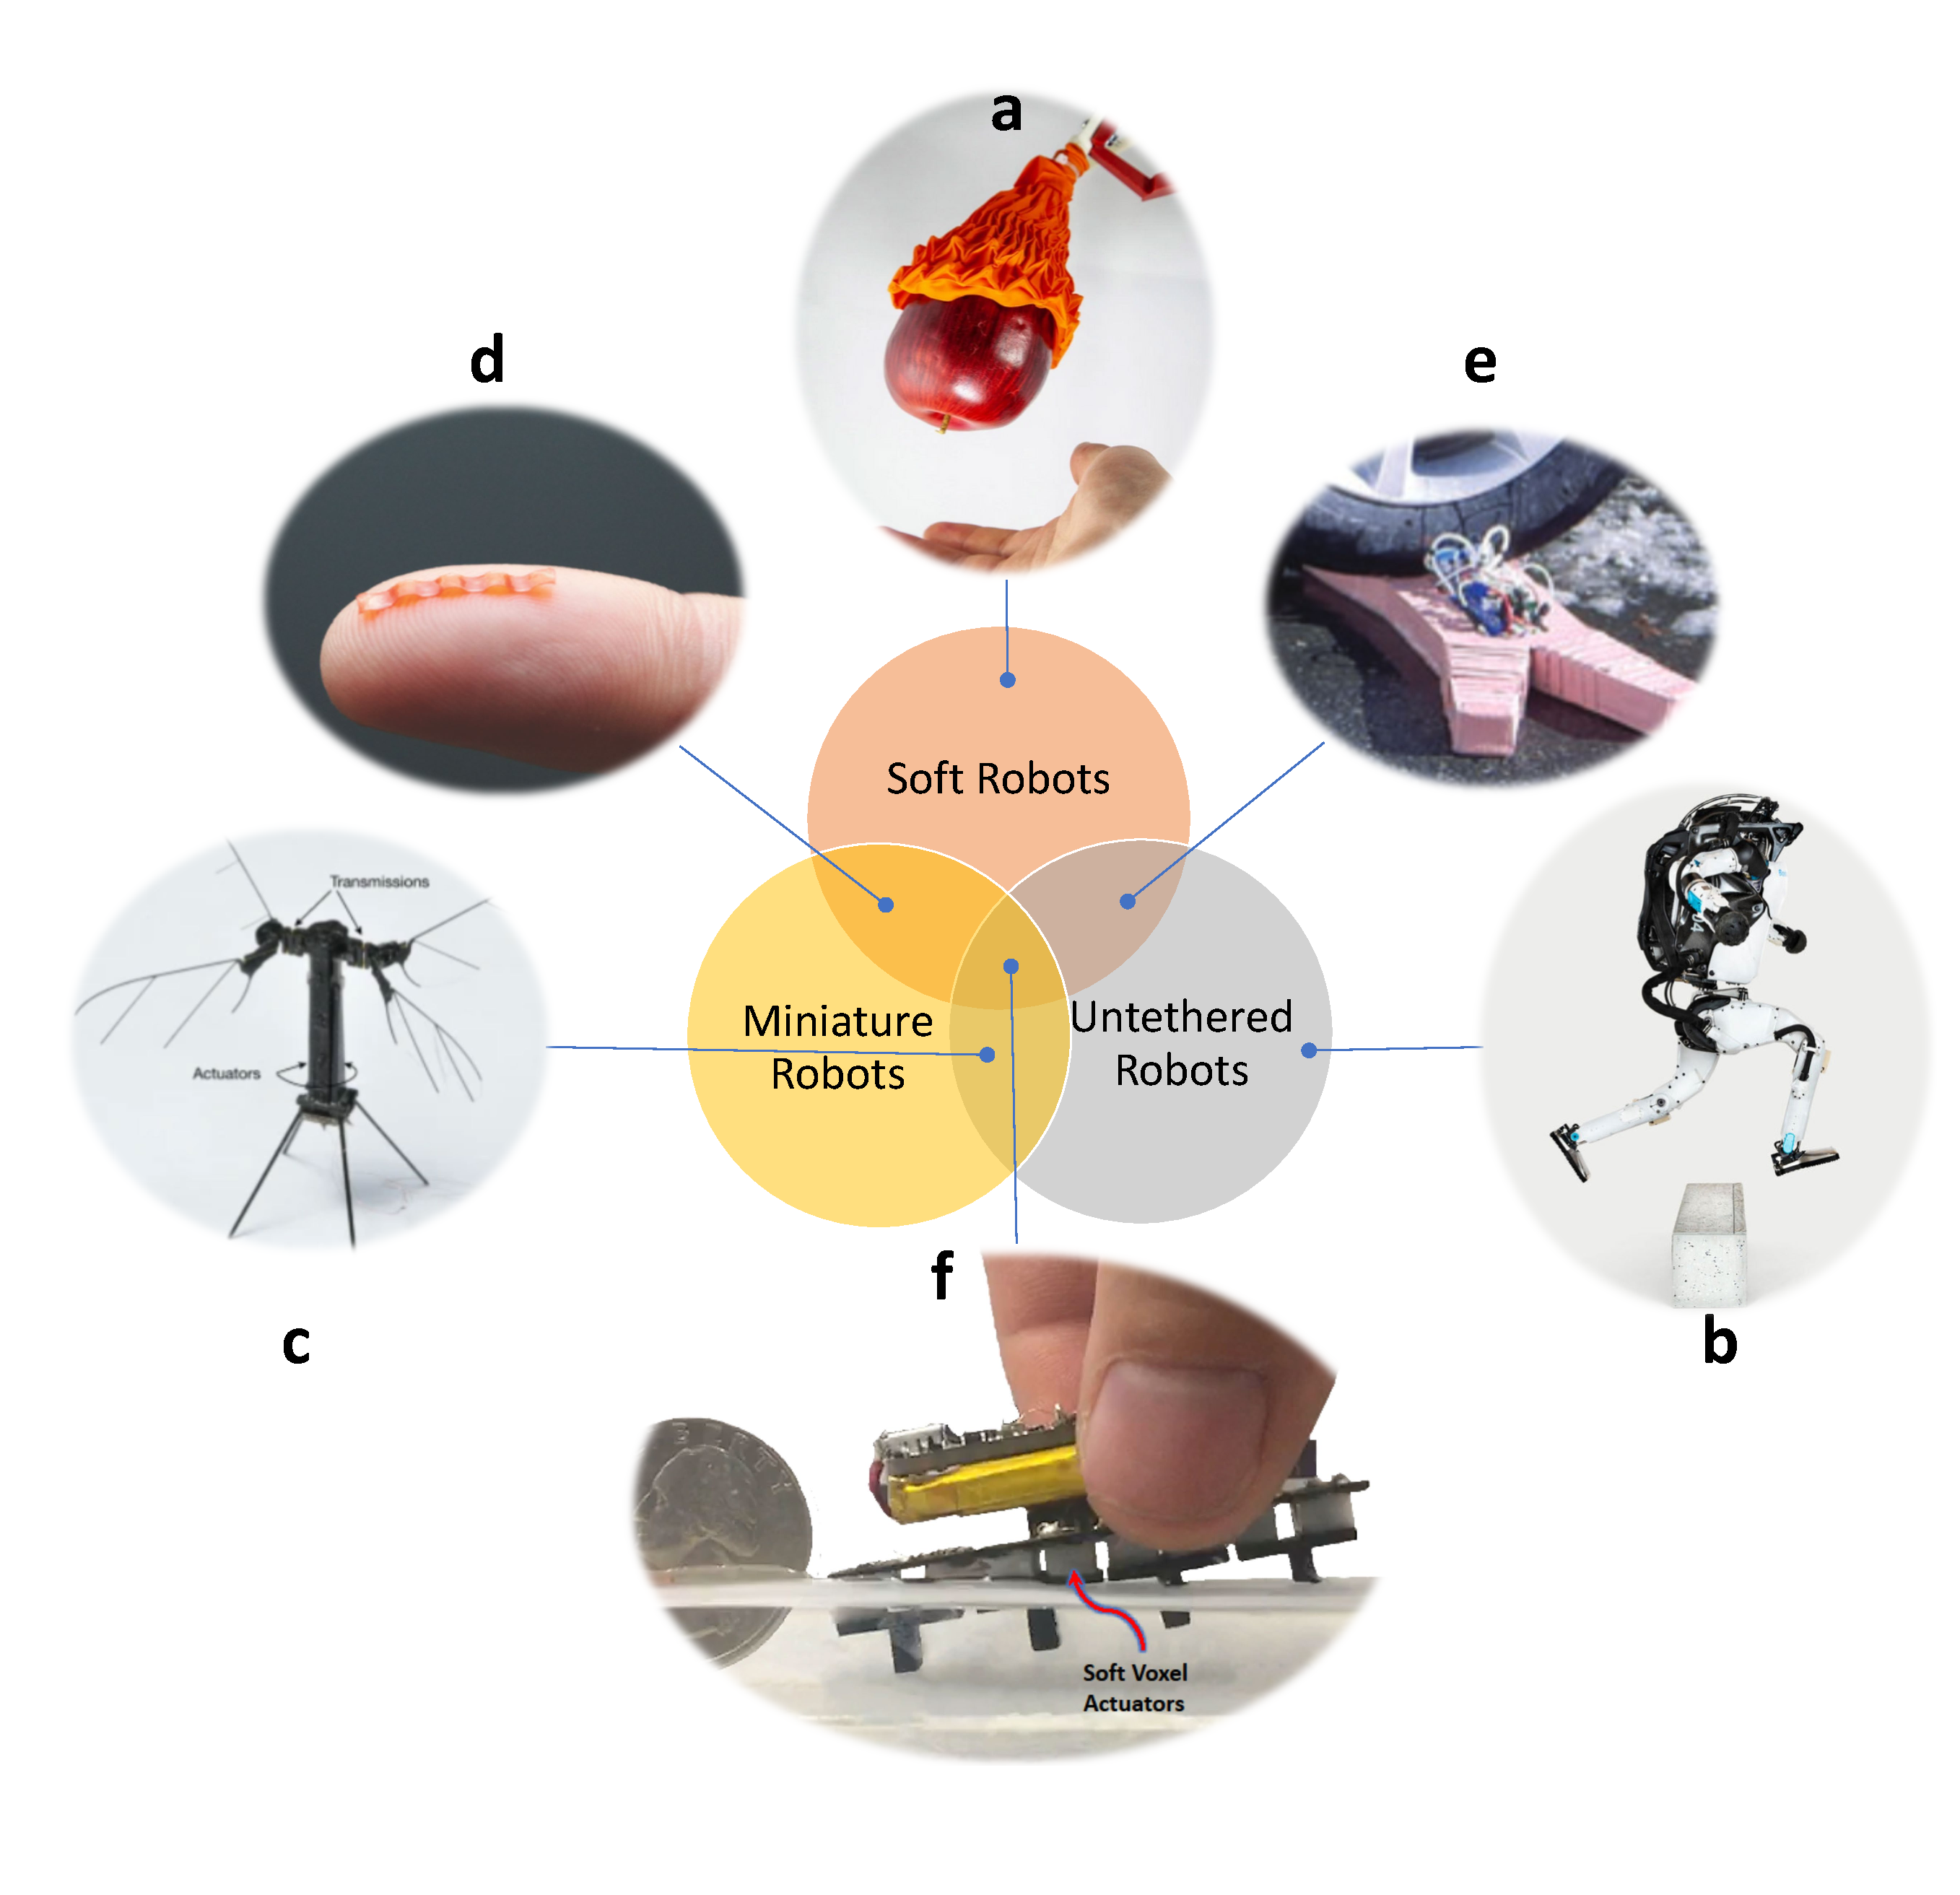
\includegraphics[width=\textwidth]{venn.pdf}
      \caption[\capitalisewords{Classification of robots.}] {a) soft robot~\cite{Li2019}. b) Untethered robot~\footref{fn:boston} c) Miniature untethered robot~\cite{Jafferis2019} d) Miniature soft robot~\cite{Tingting2012} e) Untethered soft robot~\cite{Tolley2014d} f) Miniature untethered soft robot~\cite{Khodambashi2021untethered}}
      \label{fig:venn}
\end{figure*}

\section{Soft Robotics as an Emerging Field}
\label{sec:emerging}
The majority of biological organisms consist of soft tissue, which provides some advantages to these biological systems. The octopus is the most widely used cited source of inspiration for soft robotics research because of their capabilities; they can deform their body and pass through small openings. Therefore, shape morphing is one of the key advantages of soft organisms. Octopuses can also soften their arm as they wrap it around a bottle cap and stiffen their arms for a tight grip as they turn the cap to open it as shown in \textcolor{red}{Fig}. Variable stiffness is therefore, another aspect of soft organisms. The human hand is another example of a soft system that can demonstrate some of the advantages of compliant materials; it can grasp objects across a wide range of shapes and surface roughnesses without slipping because the soft tissue surrounding the skeletal system passively conforms to different shapes, improving conformance, increasing the contact surface area, and permitting higher forces to be passed to the grasped object \textcolor{red}{(Fig)}. The human hand can also absorb energy from impacts, as it does when catching a baseball, absorbing energy and reducing the risk of damage. The ability to absorb impact energy also protects the surrounding objects and humans in case of a collision. This brings up safety as another important feature of compliance present in soft bodied animals  that can be important in the design of soft robots. The advantages of soft animals are summarized in \textcolor{red}{Table}. Inspired by biology, soft robot developers try to utilize the advantages inherent in soft, compliant matter to achieve safer interactions around humans or more robust locomotion and manipulation in unstructured environments~\cite{martinez2013,laschi2012,Tolley2014d,AdamBilodeau2015}.	

\section{\capitalisewords{State of the Art in Soft Robotics}}
Early robots were designed to be stationary. They were unaware of their surroundings and operated based on a prescribed set of instructions. Recent advances in sensing has paved the way for to mobile, autonomous, untethered robots. In addition to soft actuators, soft sensors and soft computers are thus an integral part of untethered robotic systems. For soft robots, ideally all these components are soft. With special attention paid to soft actuators --which is the focus of this dissertation-- the state of the art technology in each category (untethered, soft, miniature robots) is reviewed. 
%Soft robots are categorized based on many different features. Here, we focus on miniature and untethered robot categorization to stay focused on the topic of this thesis. Since manufacturing is part of the contribution of this thesis, a brief survey of the manufacturing techniques is also presented.
%\subsection{Components of a Soft Robot}
\subsection{Soft Sensors}
Research on soft sensors focuses mainly on stretchable sensors for wearable health monitoring~\cite{Liu2017c,Amjadi2016a}. Since these sensors exhibit characteristics, researchers have focused on solutions for integrating soft sensing into soft robotic systems. Sensors based on liquid metals have been successfully implemented within soft structures to measure strain~\cite{Hammond2014,Chossat2013, Wang2019c,Ren2020}. Other sensor technologies include piezoresistive~\cite{Georgopoulou2020,Turgut2018,Melnykowycz2016}, capacitive~\cite{Hohimer2020,Cao2020,White2017,Frutiger2015}, and conductive polymers~\cite{Chen2021,Kanoun2021,Harito2020} which rely on the change in resistance or capacitance of the material when they undergo strain. 
\subsection{Soft Computers}
Traditionally, the majority of computation in robotic systems is performed by microcontrollers made of hard materials. This is unavoidable and is one of the major limiting factors in the development of entirely soft robots. Soft computers are in their incipient stage; they are based on pneumatic networks and have been demonstrated performing simple logic functions~\cite{Preston2019,Garrad2019}. Another research direction uses living cells as computers~\cite{Daniel2013}. In general, the topic of soft computing requires significant development before it can be successfully implemented within soft robotic structures. 
\subsection{Soft Actuators}
Actuators are often the core of robotic designs, and as such, there is a larger amount of research on soft actuators compared to soft sensors and computers. Soft pneumatic actuators (SPAs) \cite{Gorissen2017, Branyan2018} are the most widely used category of actuators in soft robotics. Their function is based on chambers made of soft materials that are pressurized using fluids such as air or water. As a result  of pressure supplied from external supply lines, the chamber deforms and produce motions such as bending, elongation or twisting. SPAs have high power to weight ratios and exhibit a relatively fast response.  Another class of actuators use active materials whose strain is based on an externally-applied stimulus such as heat, light or magnetic field. This class includes shape memory alloys (SMAs)\cite{Cianchetti2014}, dielectric elastomer actuators (DEAs)~\cite{Carpi2008,Gu2017}, liquid crystal elastomers (LCEs)~\cite{Kularatne2017,Yu2015a}, and stimuli-responsive hydrogels~\cite{Calvert2009,Liu2020,Ionov2014,Banerjee2018}. 
 
%\subsection{Untethere d Soft Robots}
%For functioning as mobile robots, the essential accessories such as pumps or power supplies need to be embedded in the robot itself. These robots fall under the category of untethered soft robots [].  
%\subsection{Miniature Soft Robots}
%Miniature robots have dimensions under...and have a low load carrying capacity. These robots have applications where small loads need to be applied, in working with delicate objects, or in tight environments such as inside human body. 
%\subsection{Miniature Untethered Soft Robots}

%\subsection{Soft Robot Manufacturing Techniques}
%\subsubsection{Molding}
%\subsubsection{3D Printing}
\section{\capitalisewords{Challenges Ahead}}.
%\textcolor{red}{The challenge at the time those works were published was to understand the mechanisms behind shape shifting in nature and to create methods to achieve similar shape shifting in artificial matter. Recently this trend is changing, as higher demand is put towards re-programmable soft matter (as opposed to one time programmable). Hydrogels being a good candidate, they quickly found their way for these applications. Currently, the challenge is to create on-demand shape changes in a hydrogel structure, which we are trying to address in this paper. Demonstrations seen in the majority of the publications we surveyed such as {Liu, Y., et. al (2017). Sequential self-folding of polymer sheets. Science Advances, 3(3), 1–8} and {Nojoomi, A., et. al. (2018). Bioinspired 3D structures with programmable morphologies and motions. Nature Communications, 9(1), 1–11} and the work of Klein and Kim mentioned by the reviewer are shape changes by hard-coded structures. These papers, although they mention robotics as one of the main application areas of hydrogels, do not demonstrate any object manipulation, interaction with the environment or robotic functions. In Figure 3A, we show that using our approach, it is possible to create similar hard-coded structures. The difference is that by introducing the hydrogel voxels as building blocks, our structures can be produced in a significantly simpler way (manually in the present work and automatically using voxel printers in the future work) --a key feature that is highly demanded in the soft robotic community. 
%In this dissertation, enabling technologies and simultaneous innovations in the areas of material synthesis, processing and manufacturing  is introduced as opposed to other research which usually focus only on one of the areas. These innovations resulted in a hydrogel that has fast response, tunable response, rapid polymerization time (under 10 seconds) and uses cheap and readily available ingredients (DI water). While in the prior work we surveyed, only some of the features have been achieved at a time. We have combined these features with voxel-based manufacturing, which facilitates material distribution and placement of actuators. Although we have used hydrogels for producing the voxels, the range of materials that can be used using this method is wider compared to 3D printing or lithography methods. These contributions are manifested through our demonstrations which present a class of heterogeneous hydrogel structures with unique capabilities not demonstrated previously in the literature. These capabilities are on-demand dynamic shape changes which allows the structures to interact with unstructured environments. In other words, without these innovations, the demonstrations would not be possible. Therefore, we think our proposed methods which are developed through cross functional collaboration of material scientists and roboticists satisfy multiple requirements that a material needs to have to be widely accepted for soft robotics applications. This can be considered as our main contribution on top of others.}
The focus of early soft robots was to identify methods for manufacturing and assembling SPAs and assemble them into functioning prototypes. These early soft robots were created for tasks such as grasping or were used as stationary continuum manipulators. In these applications, the size and weight of the supporting fluidic equipment was not important because they could be located near the robot and did not have to be transported. In case of mobile robots, however, all the supporting equipment must be included within the robot, and therefore, careful design is required to meet payload limitations. This challenge becomes more pronounce in the case of miniature robots where there is less space available within their body to include all the accessories. SPAs use passive soft materials such as silicone elastomers for pneumatic actuation and rely on rigid components such as motors and pumps for providing fluidic power; these devices are difficult to scale to millimeter or micrometer-scale robot designs and therefore, manufacturing small-scale soft actuators for applications such as healthcare, wearable devices, manufacturing, and robotics as envisioned by \cite{Hines2017} has remained a bottleneck in the development of miniaturized soft robots \cite{Majidi2019}. This category of soft robots has been the least explored due to this issue, as well as the complexity of scaling down soft fabrication techniques. Though small-scale actuators can be produced using responsive materials such as DEAs, LCEs and hydrogels, these actuators lack sensing and computation, which are essential subsystems of a true robot. These systems are thus usually used in a human-in-the-loop scenario, where sensing and computation are performed by a human operator. This helps in down scaling the robots to the micrometer range. These actuators can perform limited robotic functions and have highly specific applications such as to perform a colon tissue biopsy. However, these robots can not function as autonomous robots because they lack sensing and computation and rely on external devices for their operation. For instance,~\cite{Palagi2016} needs a light projecting device to generate the light patterns required for creating deformations and movement in a light-responsive actuator. Another example is a magnetic-responsive actuator~\cite{Kim2018} which rely on a magnetic field generator for its operation. All these equipment are bulky and require careful setup and therefore, these types of actuators are not suitable for use in autonomous mobile robots. Technologies are still needed to create small-scale autonomous soft robots that function similar to biological organisms such as annelids, mollusks, and octopuses. Considering the highly sophisticated structure of living organisms, simultaneous progress in multiple disciplines such as materials science, design, manufacturing and control is required in order to achieve soft robots that are closer to their biological counterparts.
The focus of early soft robots was to identify methods for manufacturing and assembling SPAs and assemble them into functioning prototypes. These early soft robots were created for tasks such as grasping or were used as stationary continuum manipulators. In these applications, the size and weight of the supporting fluidic equipment was not important because they could be located near the robot and did not have to be transported. In case of mobile robots, however, all the supporting equipment must be included within the robot, and therefore, careful design is required to meet payload limitations. This challenge becomes more pronounce in the case of miniature robots where there is less space available within their body to include all the accessories. SPAs use passive soft materials such as silicone elastomers for pneumatic actuation and rely on rigid components such as motors and pumps for providing fluidic power; these devices are difficult to scale to millimeter or micrometer-scale robot designs and therefore, manufacturing small-scale soft actuators for applications such as healthcare, wearable devices, manufacturing, and robotics as envisioned by \cite{Hines2017} has remained a bottleneck in the development of miniaturized soft robots \cite{Majidi2019}. This category of soft robots has been the least explored due to this issue, as well as the complexity of scaling down soft fabrication techniques. Though small-scale actuators can be produced using responsive materials such as DEAs, LCEs and hydrogels, these actuators lack sensing and computation, which are essential subsystems of a true robot. These systems are thus usually used in a human-in-the-loop scenario, where sensing and computation tasks are performed by a human operator. This can make it possible to scale soft robots to micrometer ranges, though resulting actuators can perform limited robotic functions and have highly specific applications such as to performing colon tissue biopsies. Because of the sensing and control limitations of small-scale microrobots, such systems, cannot truly function as autonomous robots and rely on external devices for their operation. For instance, the sof microrobot made of LCE described in~\cite{Palagi2016} requires a light-projecting device to generate the light patterns required for creating deformations and movement in a light-responsive actuator. Another example is the magnetic-responsive actuator used in~\cite{Kim2018} which relies on a magnetic field generator for its operation. This equipment is universally bulky and requires careful setup and comlex computation. Therefore, these types of actuators are not suitable for use in autonomous mobile robots. Technologies are thus still required that enable small-scale autonomous soft robots which function similarly to biological organisms such as annelids, mollusks, and octopuses. Considering the highly sophisticated structure of these organisms, simultaneous progress in multiple disciplines, such as materials science, design, manufacturing and control is required in order to achieve soft robots that are closer to their biological counterparts.

Hydrogels are close to soft tissue in terms of their material properties and the muscle-like contractions in response to external stimuli~\cite{Liu2020}. They can be tuned to be ion conductive as well as biocompatible. These attributes can help hydrogel soft robots address the core benefits of soft devices namely safety and adaptability~\cite{Lee2020}. However, the uniform responsive volume change of bulk hydrogels makes them less interesting in robotic applications, which demands complex spatiotemporal reconfigurability~\cite{Erol2019} - as the dexterity of the octopus's arm demonstrates. 

In summary, the challenge for small, untethered soft robots is to create 1) on-demand, 2) time-varying, 3) local deformations in a hydrogel structure. From a structural design perspective, the majority of reported heterogeneous hydrogel structures made up till now demonstrate fixed deformation patterns, such as static shape shifting of sheets, without any interaction with the environment~\cite{SydneyGladman2016, Ma2019, Jeon2017}, or bending of beams to perform simple gripping functions~\cite{Wang2017, Ma2018, Duan2017}. Only a few methods demonstrate on-demand deformations for interacting with objects~\cite{Mourran2017, Palagi2016, Kim2018}; these approaches, however involve bulky equipment (light and magnetic field generators), making them impractical for mobile soft robots or embedded applications.
From a materials perspective, there is a need for a powerful but simple synthesis method to broadly tune the material response behavior (volume changing ratio, speed, and stiffness), to meet the requirement of creating a complex robotic structure with spatiotemporal reconfigurability.

\section{Contributions of this Dissertation}
This dissertation demonstrates progress in different areas of material science and manufacturing  that together contribute to the field of soft robotics. A set of design decisions are made based on close collaboration with teams of material scientists and roboticists which helps inform progress of one field by considering the requirements of the other. 

A bioinspired approach is applied in several design decisions. Biological organisms use electrical signals from the nervous system in conjunction with responsive muscle tissue to perform soft actuation. This combination helps them to be self-contained and also, it is viable across scales from giant octopuses to millimeter-sized worms. Therefore, the first feature that is considered for the design of soft robots is to use a material that is responsive to electrical stimulus. The living organisms also are made of cells which are simpler building blocks assembled to form a more complex organ. The second requirement imposed is therefore, to use a bottom-up strategy to fabricate complex robots using simple building blocks that are easy to manufacture. 

The contribution of this dissertation, as shown in Figure~\ref{fig:summary}, can be summarized as follows:

\begin{itemize}
	\item A novel, temperature-responsive hydrogel material with fast response. This material functions as artificial muscle tissue. 
	\item A facile and tunable synthesis method for making soft actuators that is accessible to the soft robotics community, where in-house material synthesis, training, and capability, is more limited than in material-science focused lab spaces.
	\item A voxel-based assembly approach that uses simple building blocks called soft voxel actuators (SVAs) in the assembly of more complex soft robots. SVAs are easy to manufacture and solve some of the challenges associated with embedding electronics in soft robots.
	\item The use of electrical Joule heating of SVAs in the generation of a motion/force response. This enables the use of small-footprint microcontrollers and paves the way to embedded and mobile robot applications.
	\item Realization of hyper-redundant, hydrogel-based, electrically-addressable, miniature soft robots capable of performing tasks that require high degrees of freedom. High dexterity combined with the ability to function in unstructured environments separate our soft robots from previously demonstrated ones.
	\item Realization of miniature untethered soft robots that weigh only 20g including battery and power supply and does not rely on external equipment or human intervention for its operation.
\end{itemize}
\begin{figure*}[!ht]
      \centering
      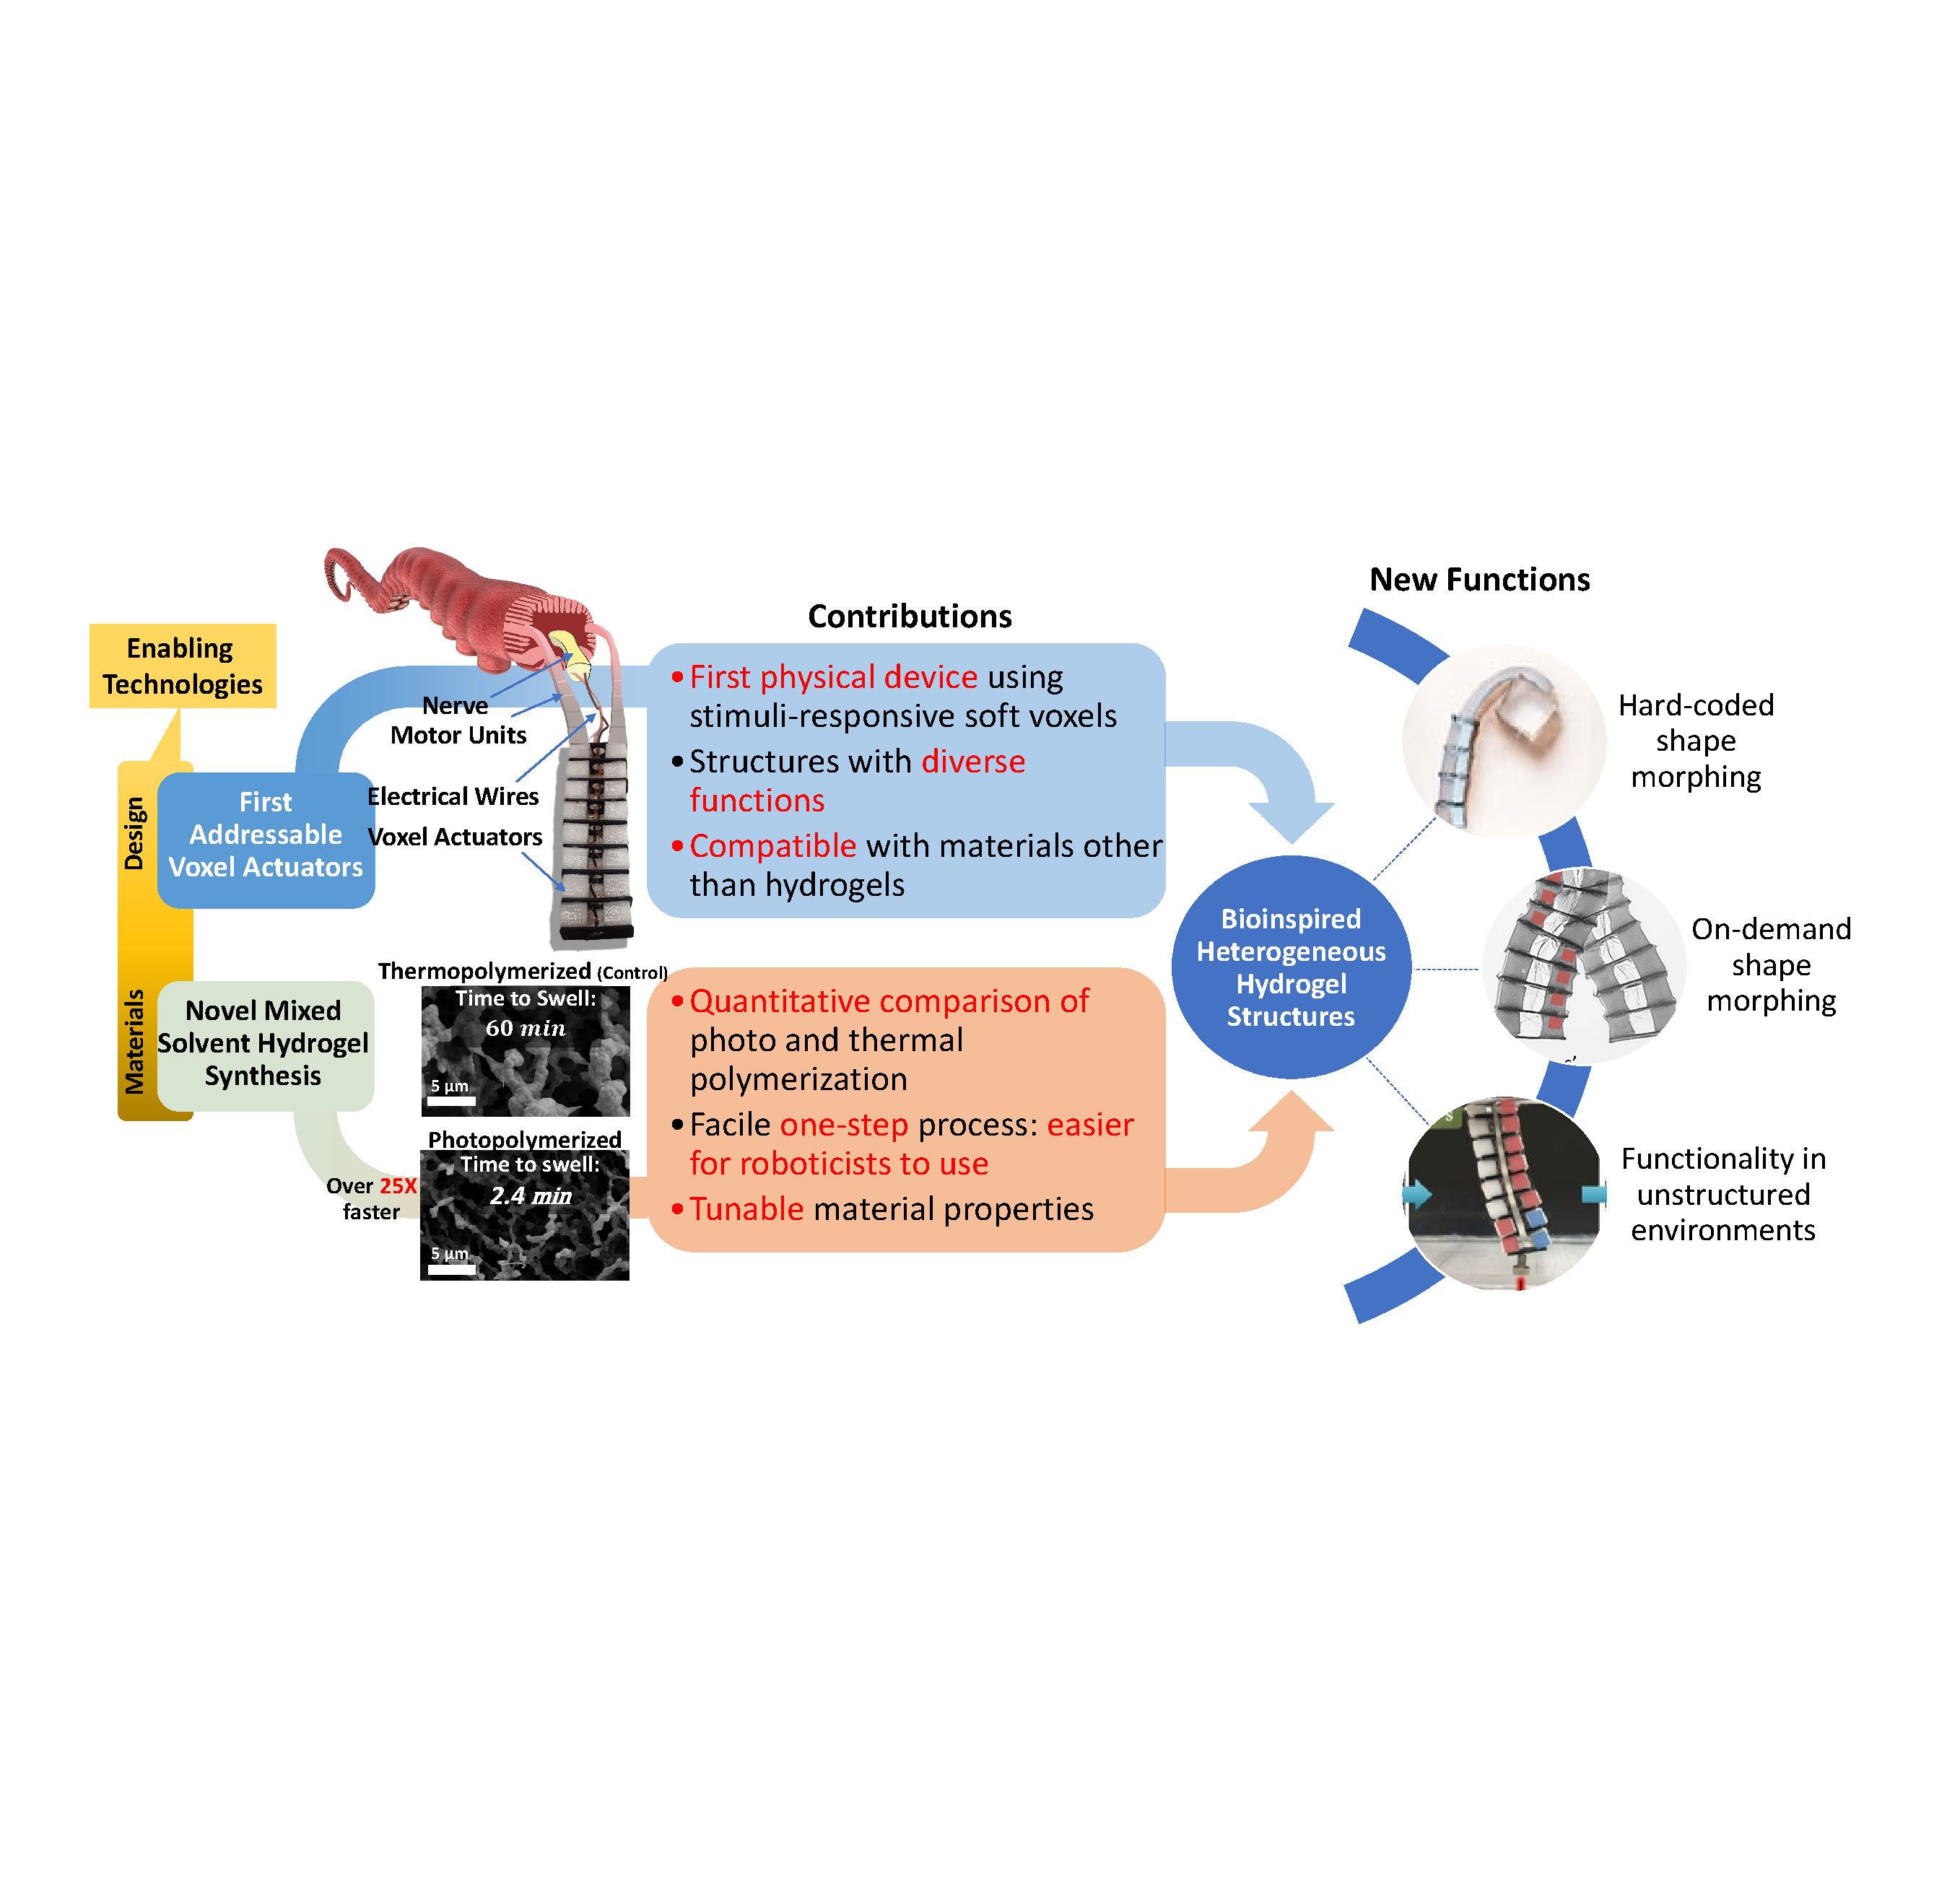
\includegraphics[width=\textwidth]{summary.pdf}
      \caption[\capitalisewords{Summary of contributions of this dissertation}]{}
      \label{fig:summary}
\end{figure*}
%\subsection{Broader Impact}
%\subsubsection{Scientific}
%Current soft actuators rely on additional hardware such as pumps, high voltage supplies, light generation sources and magnetic field generators for their operation. These components resist miniaturization and embedding them into small-scale soft robots would be challenging. This limits their mobile applications especially in hyper-redundant robots where a high number of actuators are needed. On the other hand, our developed SVAs weigh only 100 mg and require small footprint microcontrollers for their operation which can be embedded in the robotic system. 
%\subsubsection{Social}
%Soft robots are intrinsically safe around humans. This can help bring robots to daily life applications such as household robots and assistant robots for elderly people. Also, our soft robots can operate underwater due to hydrogel compatibility with moist environments. A swarm of soft robots can be used for underwater exploration and data collection and help monitor the climate change through recording the water current temperatures over long period of time.

\subsection{Dissertation Outline}
The following chapters discuss the innovations in materials science and manufacturing methods that lead to the development of miniature untethered soft robots.\\ 
\textbf{Chapter~\ref{chap:SVAs}: Soft Voxel Actuators: Hydrogel Building Blocks for Bottom-up Assembly of Soft Robots}\\
This chapter discusses the recipe for preparing temperature-responisve hydrogels. Improvements have been made in the synthesis technique such that it is more accessible to robotic researchers who have less access to material processing facilities. In addition, this recipe results in hydrogels with fast response, solving a challenge that has limited the use of hydrogels in soft robotics. Next, building blocks called soft voxel actuators (SVAs) are introduced that facilitate the manufacturing of soft robots through a bottom up assembly approach. Both the hydrogel and SVAs are characterized in-depth in terms of material properties and actuation properties.
  
\textbf{Chapter~\ref{chap:heterogeneous}: Heterogeneous hydrogel structures as Miniature Hyper-redundant Soft Manipulators}\\
This chapter is  a case study of the application of SVAs towards miniaturizing soft robots while maintaining their high degrees of freedom. Hyper-redundant miniature soft robotic manipulators are developed. It is shown that the use of SVAs enables for the first time the development of such robots. These robots are able to work in unstructured environments, where  working conditions might change. This manipulator has 16 actuators in a $40\times 10\times 4.5$~mm footprint which, is the highest reported number of degrees of freedom in a miniature robot of this size and material type.

\textbf{Chapter~\ref{chap:untetheredWalker}: Miniature Untethered Underwater Walking Robot}\\
This chapter is a second case study of the application of SVAs and is focusing on the development of untethered miniature robots. This chapter demonstrates that SVAs can significantly reduce the weight and size of such robots, without limiting payload. These robots are fully untethered which means all the electronics and batteries are carried by the robot. 

\textbf{Appendix~\ref{chap:control}: Tracking Control of a Miniature 2-DOF Manipulator with Hydrogel Actuators}
The electrical stimulation of SVAs inspired by biology has many advantages and open the doors to equip the robots with artificial intelligence. As a first step, the automatic control of SVAs using a microcontroller is presented in this chapter. Instead of turning the SVAs on and off as explained in Chapter~\ref{chap:heterogeneous}, the deformation of SVAs are controlled using a closed-loop control system based on the feedback from vision sensors which record the desired output of the system. A 2-DOF manipulator is fabricated using two SVAs and the position of the tip of the manipulator is controlled. As a final demonstration, a starfish-inspired robot is presented which can move a payload. Closed-loop control enables faster payload transport compared to an open loop control because the trajectory that each foot follows remains near optimal despite different loads and disturbances. 

